% !TeX root = ../report.tex

\section{Appendix}
\begin{figure}[H]
    \centering
        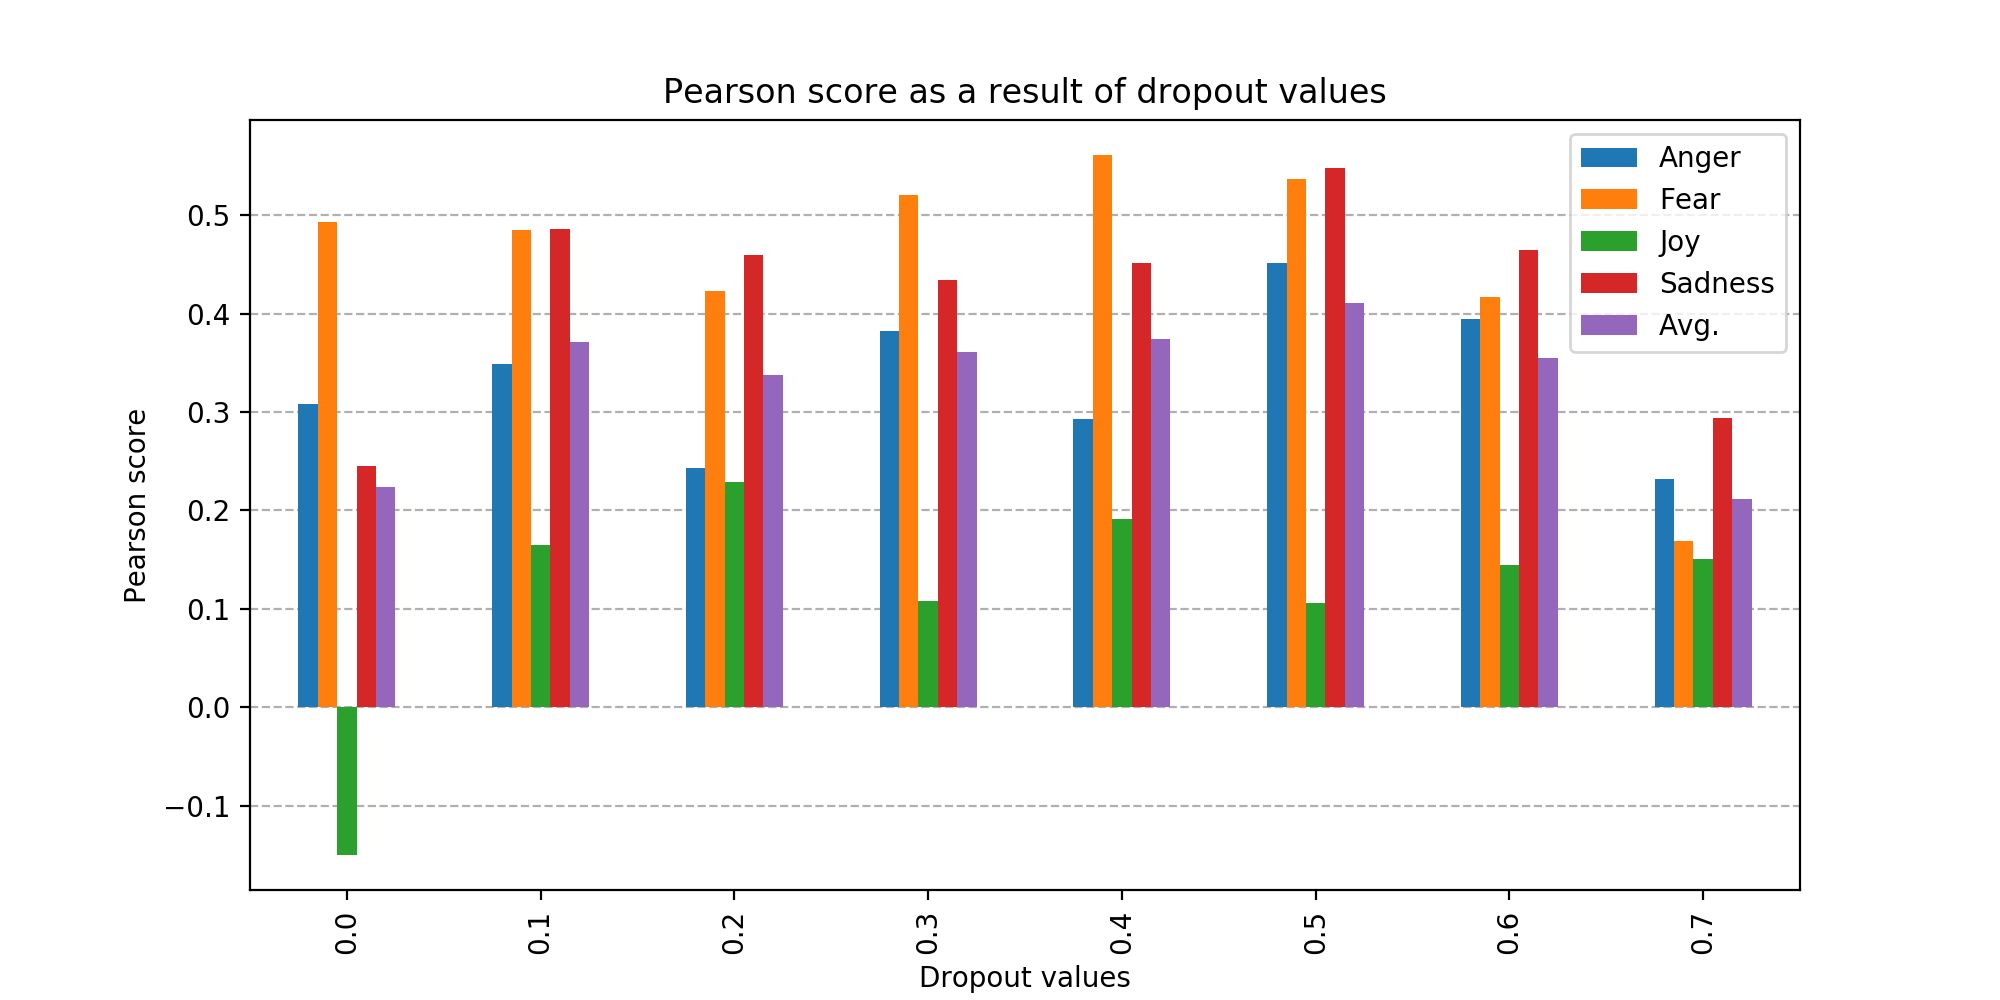
\includegraphics[width=\textwidth]{pictures/dropoutvalues.png}
        \caption{Pearson scores as a function of dropout value, loss weight set to 0.45, weighted BCE set to 0.5}
        \label{fig:dropoutvalues}
\end{figure}

\begin{figure}[H]
    \centering
        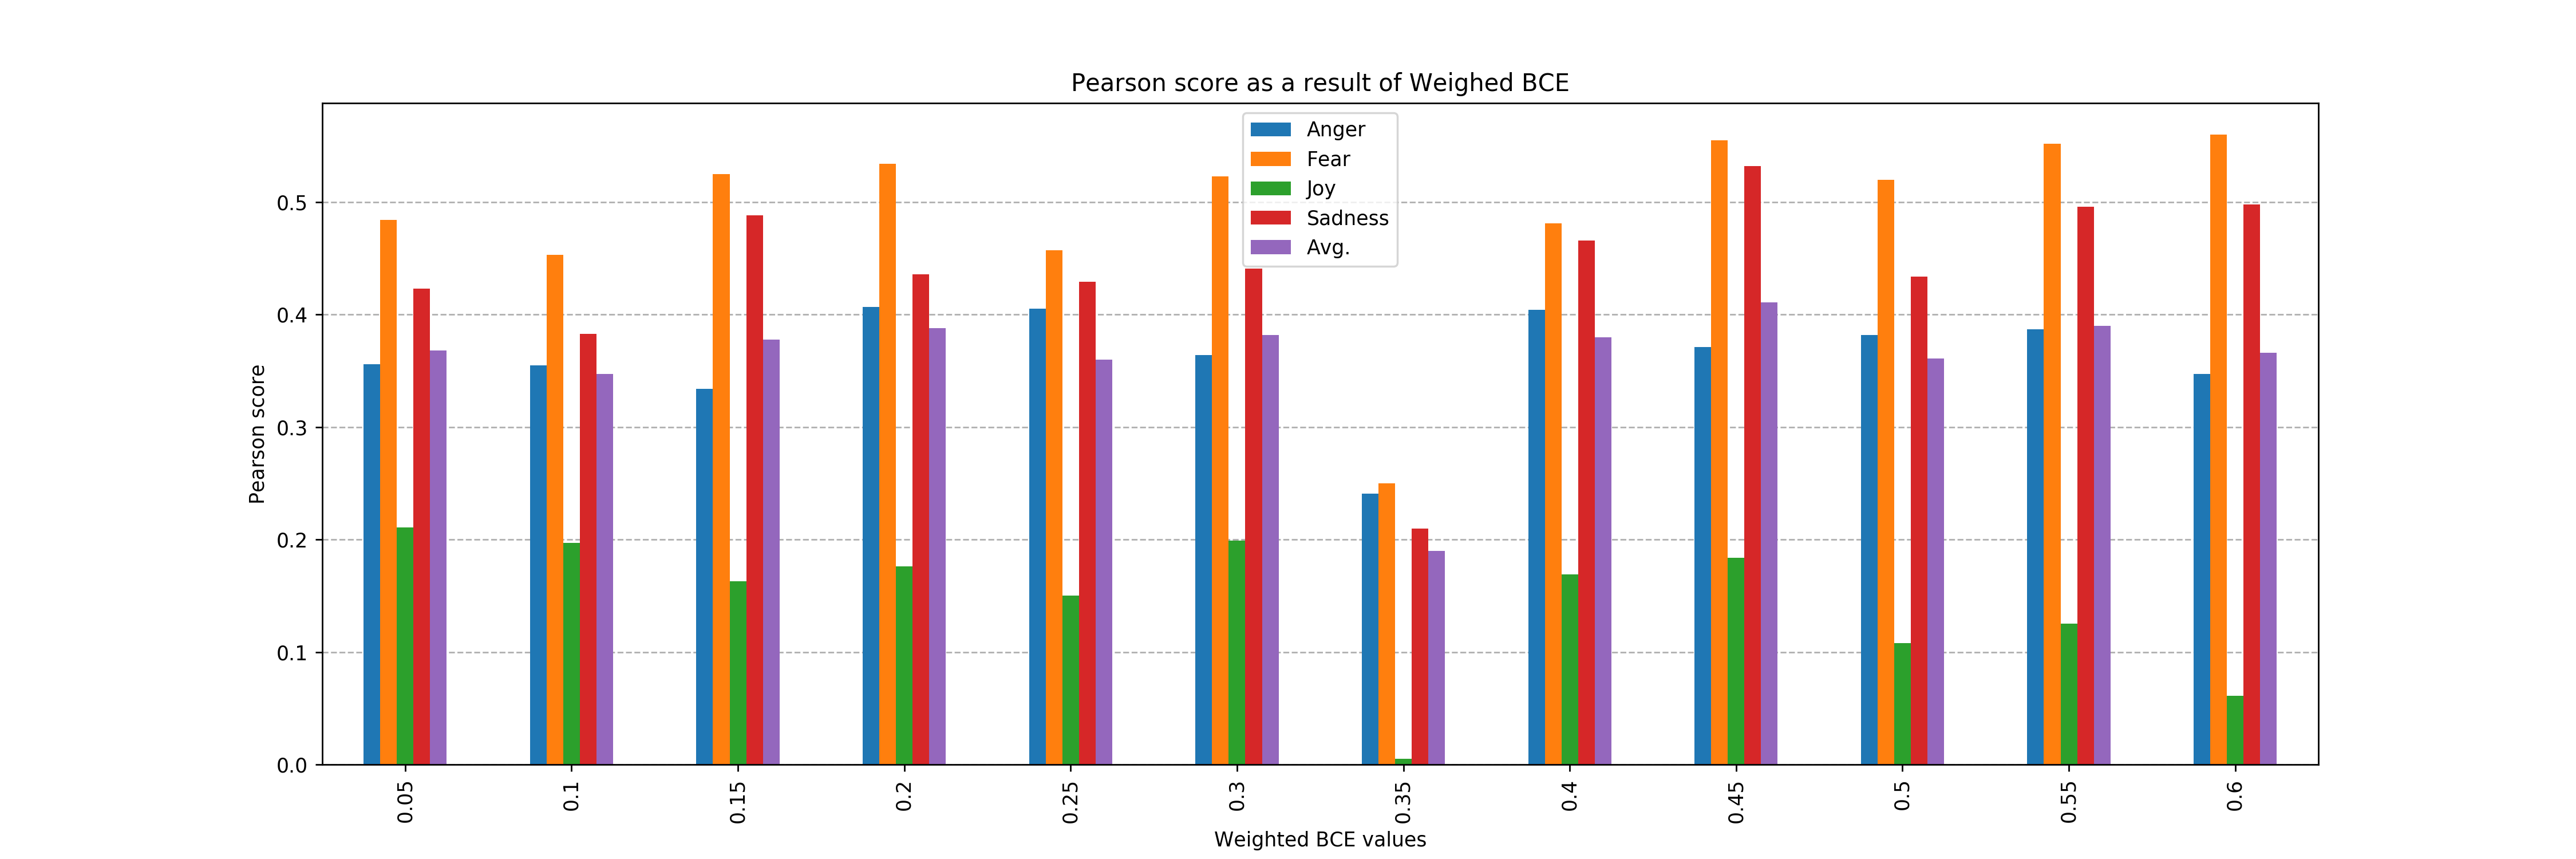
\includegraphics[width=\textwidth]{pictures/weightedBCEvalues.png}
        \caption{Pearson scores as a function of weighted BCE value, dropout set to 0.3, loss weight set to 0.45}
        \label{fig:BCEvalues}
\end{figure}

\begin{figure}[H]
    \centering
        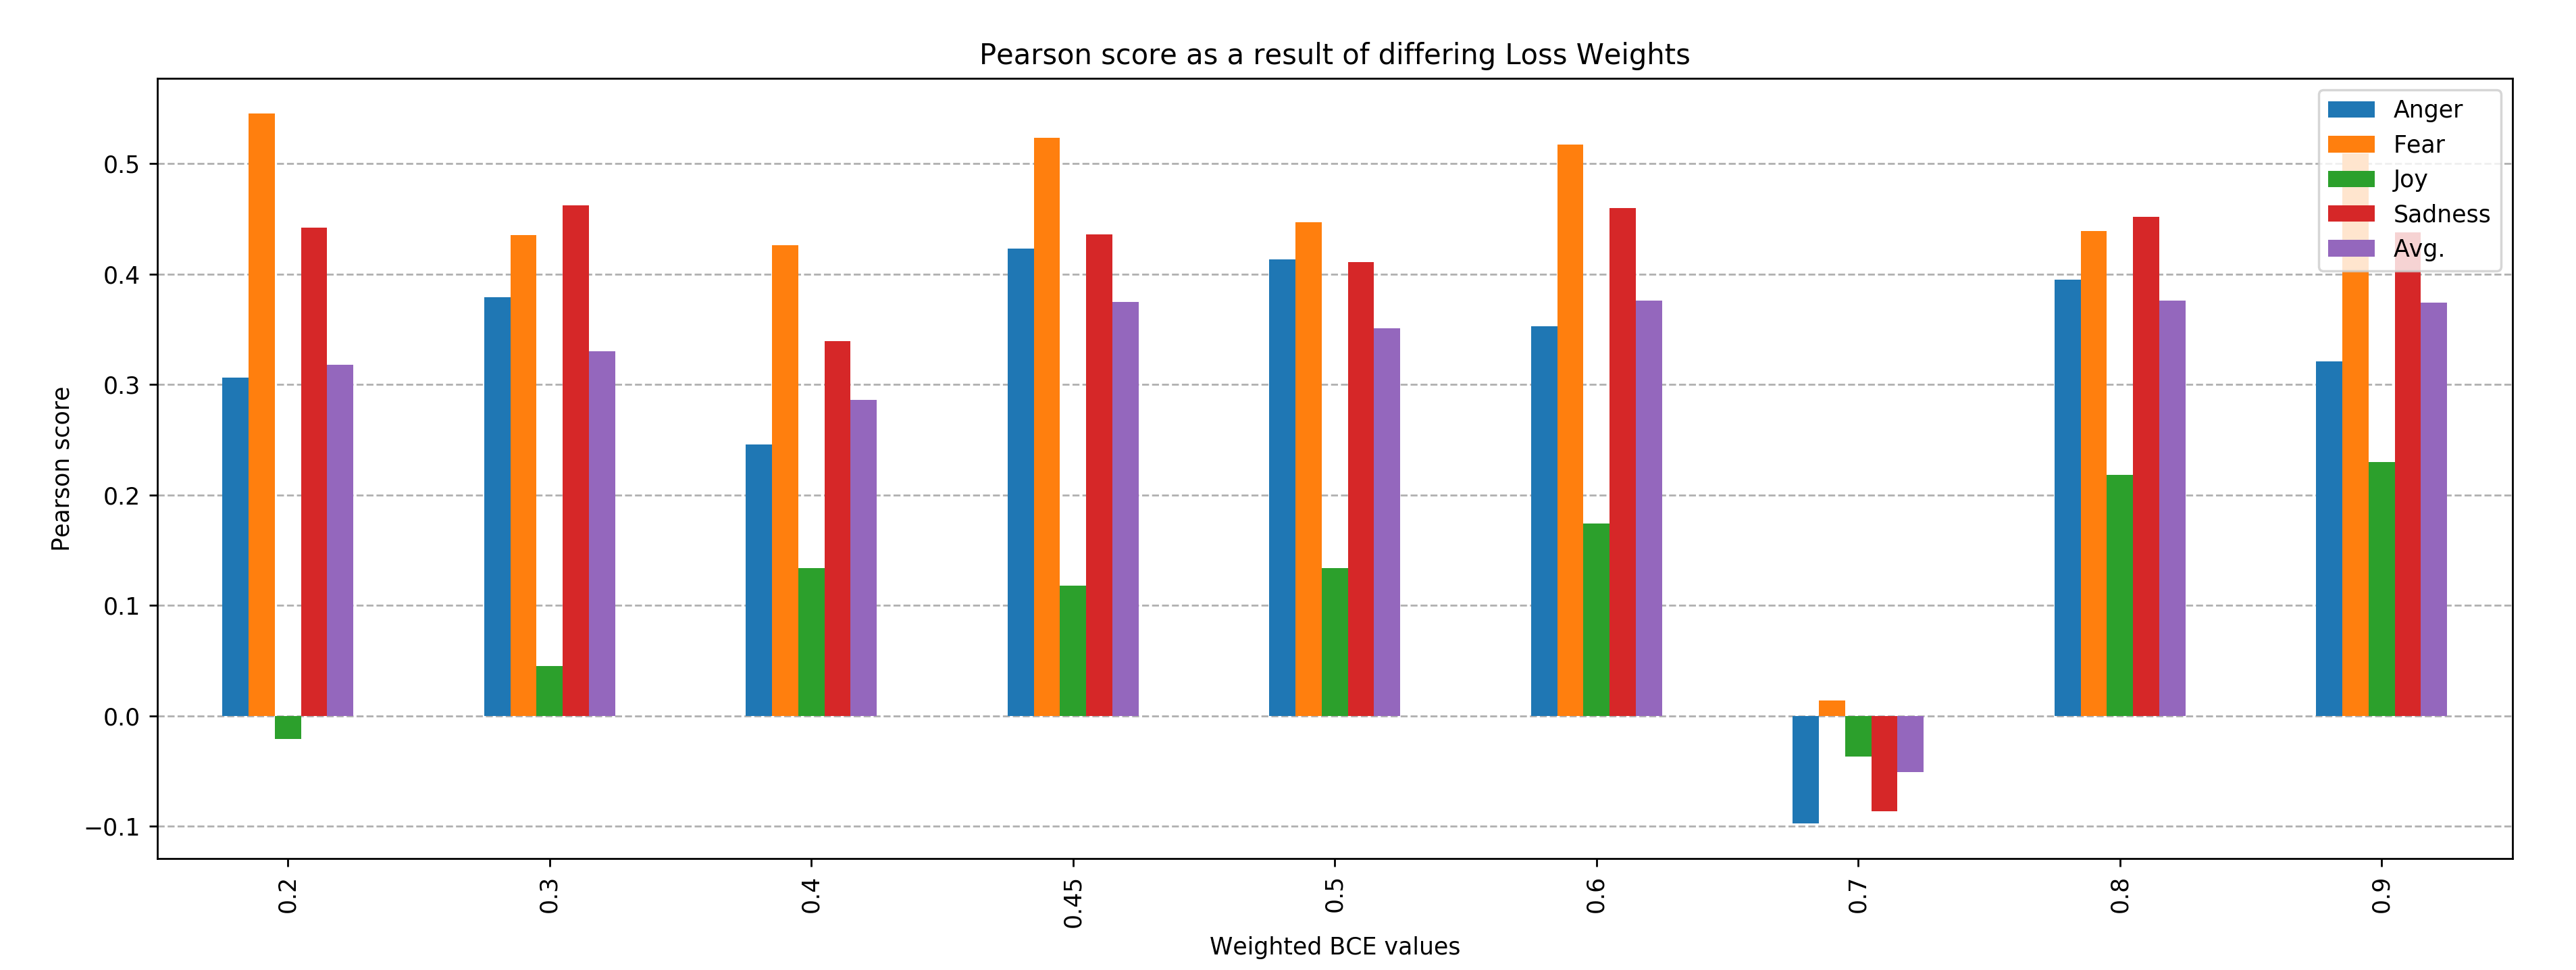
\includegraphics[width=\textwidth]{pictures/LossWeightsvalues.png}
        \caption{Pearson scores as a function of loss weight value, dropout set to 0.3, weighted BCE set to 0.45}
        \label{fig:LWvalues}
\end{figure}
